\providecommand{\main}{..}
\documentclass[\main/main.tex]{subfiles}

\begin{document}
\graphicspath{{img/}{04_hardware/img/}}
\setlength{\abovecaptionskip}{0pt}
\setlength{\belowcaptionskip}{0pt}

\chapter{Anchor hardware implementation}
In this chapter, the hardware problems relating to the anchor are discussed. The chapter starts by a brief introduction to the DWM1001 module - the main hardware for this thesis. The following sections analyze some important blocks of the circuitry for an anchor proposed by this thesis. 

\section{Introduction to DWM1001 module}
\begin{figure}[H]
    \begin{center}
        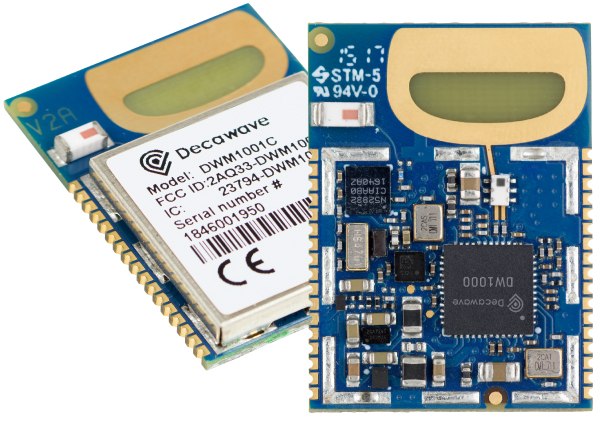
\includegraphics[width=0.3\textwidth]{DWM1001-Module_ProdPage_600x430.jpg}
    \end{center}
    \caption{DWM1001 Module}
    \label{fig:dwm1001c_module}
\end{figure}

The DWM1001 module is based on Decawave's DW1000 Ultra
Wideband (UWB) transceiver IC, which is an IEEE 802.15.4-
2011 UWB implementation. It integrates UWB and Bluetooth
antenna, all RF circuitry, Nordic Semiconductor nRF52832 and
a motion sensor.

There are multiple reasons for answering the question: why DWM1001 module is used for this thesis.
Followings are some key features:
\begin{itemize}
    \item Ranging accuracy to within 10cm
    \item UWB Channel 5 printed PCB antenna (6.5 GHz)
    \item 6.8 Mbps data rate IEEE 802.15.4-2011 UWB compliant
    \item Well known Nordic Semiconductor nRF52832 SoC
    \item Bluetooth connectivity and Bluetooth chip antenna
    \item Motion sensor is available: 3-axis accelerometer
    \item Current consumption optimized for low power sleep mode: $<$ 15$\mu$A
    \item Low supply voltage: 2.8 V to 3.6 V
    \item Small size: 19.1 mm x 26.2 mm x 2.6 mm
    \item Modules marked DWM1001C are certified to ETSI, FCC and ISED regulations
\end{itemize}

\begin{figure}[H]
    \begin{center}
        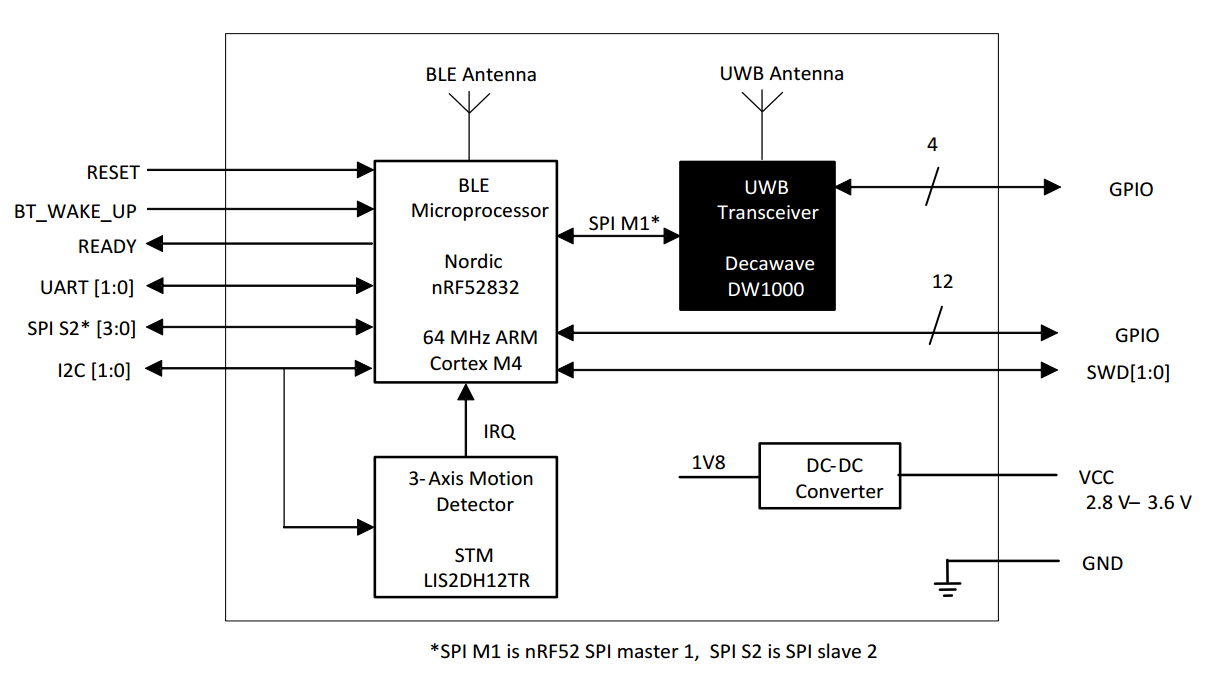
\includegraphics[scale=0.35]{dwm1001_block_diagram.png}
    \end{center}
    \caption{DWM1001 block diagram}
    \label{fig:dwm1001_block_diagram}
\end{figure}

The nRF52832 is a general-purpose multi-protocol SoC. It meets the challenges of a broad range of applications that need advanced Bluetooth LE features. It is built around an Arm® Cortex™-M4 CPU with floating-point unit running at 64 MHz. As shown in figure \ref{fig:dwm1001_block_diagram}, in the DWM1001 module, there is an nRF52832 MCU communicating to  a DW1000 radio IC over an SPI connection.

\section{Battery charger circuit}

\begin{figure}[H]
    \begin{center}
        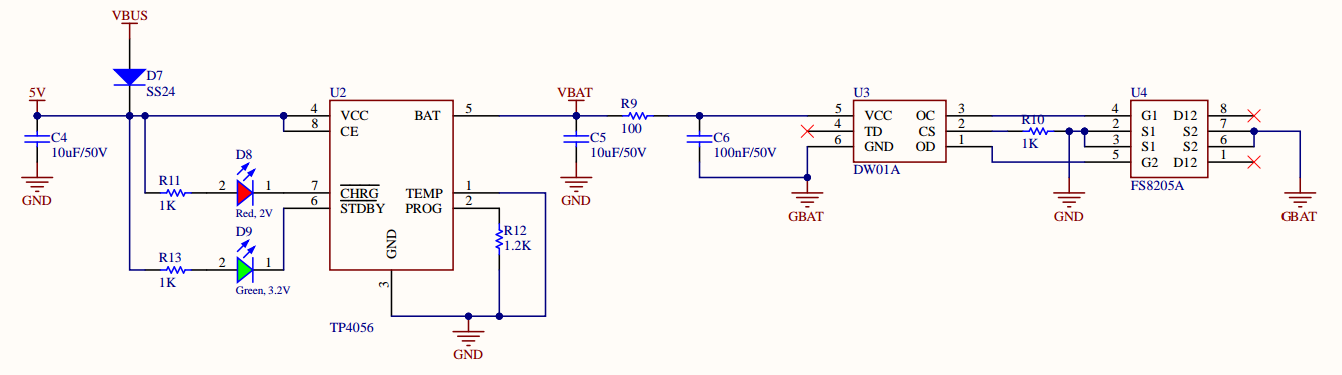
\includegraphics[width=1\textwidth]{battery_charger_circuit.png}
    \end{center}
    \caption{Battery charger circuit}
    \label{fig:battery_charger_circuit}
\end{figure}

\subsection{TP4056}

\subsubsection{CC-CV charging method}
The constant current - constant voltage (CC-CV) charging method has been extensively used for charging batteries cause it combines the advantages of both the CC and CV charging methods. As presented in figure \ref{fig:tp4056_cc_cv_profile}, the CC-CV charging method uses CC charging in the first charging stage, and when the voltage reaches the maximum safe threshold value, the charging process shifts to the CV charging method. The charging process is complete when the current levels off or when full battery capacity is reached.

\begin{figure}[H]
    \begin{center}
        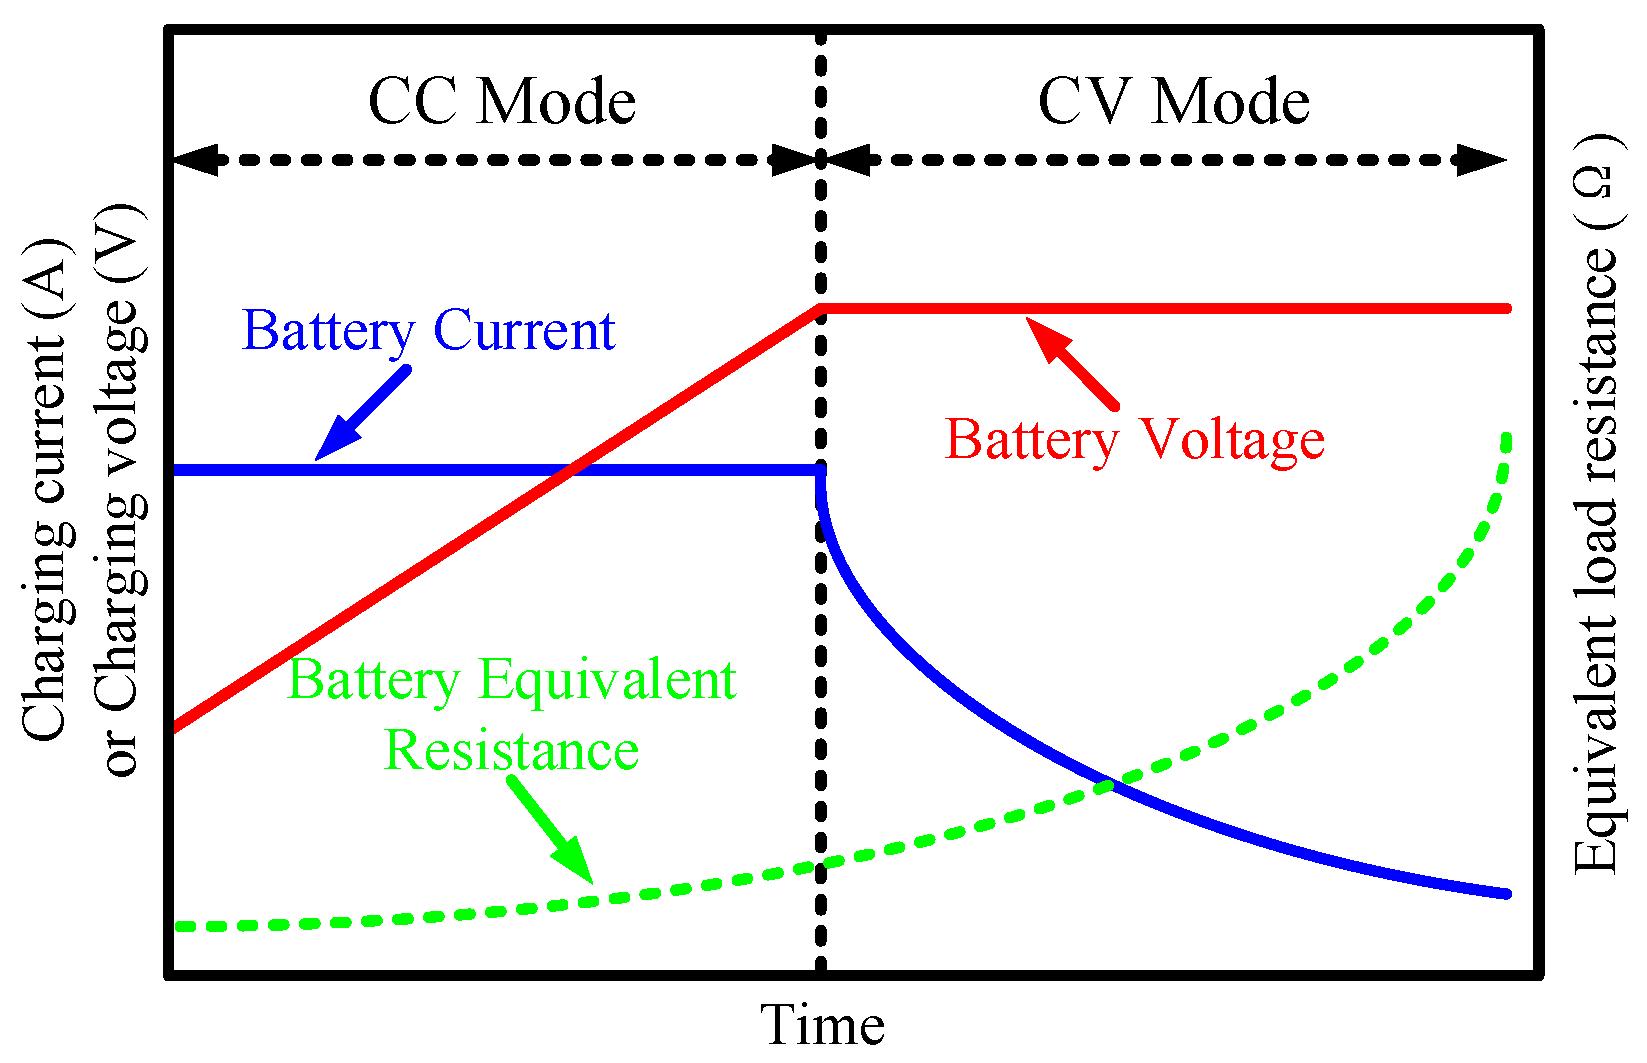
\includegraphics[width=0.6\textwidth]{tp4056_cc_cv_profile.png}
    \end{center}
    \caption{Constant current/constant voltage (CC/CV) charging profile}
    \label{fig:tp4056_cc_cv_profile}
\end{figure}

\subsubsection{CC-CV in action}
The TP4056 is a CC-CV linear charger for single-cell lithium-ion batteries. Its SOP package and low external component count make the TP4056 ideally suited for portable applications. Using TP4056, no blocking diode is required since the internal PMOSFET architecture has prevented to negative charge current circuit. The charge voltage is
fixed at 4.2V, and the charge current can be programmed externally with a single resistor. The TP4056 automatically terminates the charge cycle when the charge current drops to 1/10th the programmed value after the final float voltage is reached. 

In this thesis, the TEMP pin (Pin 1) is grounded to disabled the temperature sense function. The charge current, however, is set by connecting a resistor $R_{PROG}$ from the PROG pin (Pin 2) to GND. In this thesis, a 1.2K resistor is used for charge current setting:

\begin{equation}
    I_{BAT} = \frac{V_{PROC}}{R_{PROG}}\times 1200 = \frac{1V}{1.2K}\times 1200 = 1A
\end{equation}

Figure \ref{fig:tp4056_complete_charge_cycle} is the real profile of CC-CV charging method in the TP4056 compared to the theory profile shown in figure \ref{fig:tp4056_cc_cv_profile}.

\begin{figure}[H]
    \begin{center}
        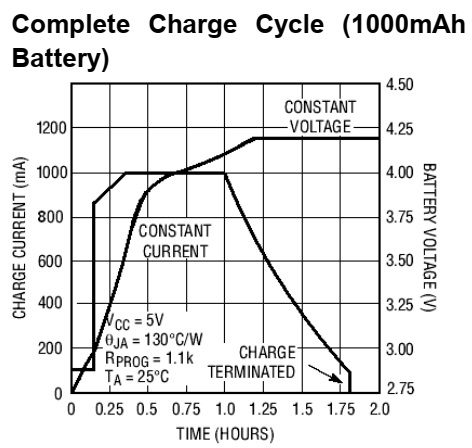
\includegraphics[scale=0.8]{tp4056_complete_charge_cycle.jpg}
    \end{center}
    \caption{TP4056 complete charge cycle}
    \label{fig:tp4056_complete_charge_cycle}
\end{figure}

\subsection{DW01A and FS8205A}

\section{Voltage step down converter}
\begin{figure}[H]
    \begin{center}
        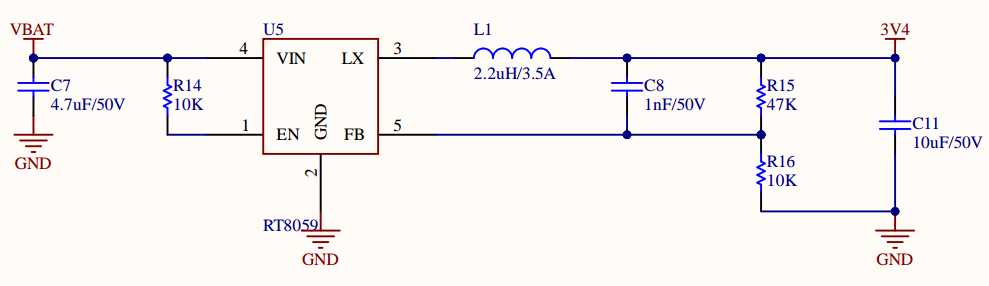
\includegraphics[scale=0.4]{voltage_set_down_converter.png}
    \end{center}
    \caption{Voltage set down converter}
    \label{fig:voltage_set_down_converter}
\end{figure}

\section{220V Solid State Relay}
\begin{figure}[H]
    \begin{center}
        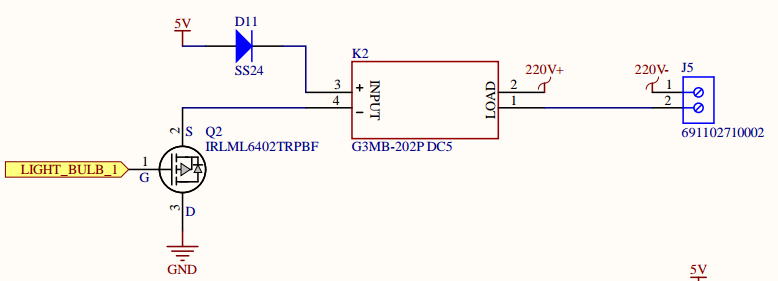
\includegraphics[scale=0.4]{relay_circuit.png}
    \end{center}
    \caption{Relay circuit}
    \label{fig:relay_circuit}
\end{figure}

\end{document}